\documentclass[11pt]{article}
\usepackage{fullpage}
\usepackage{array}
\usepackage{graphicx}
\usepackage{amssymb, amsmath}
\usepackage{hyperref}
\usepackage[labelfont=bf]{caption}

\begin{document}


\title{\textbf{Tabulation of Chemical Source Terms for Turbulent
    Combustion Simulations}}

\author{Emmet Cleary: emcleary@princeton.edu \and Daniel Floryan:
  dfloryan@princeton.edu \and Jeffry Lew: jklew@princeton.edu \and
  Bruce Perry: bperry@princeton.edu \and Emre Turkoz:
  eturkoz@princeton.edu} 

%\date{January 11th, 2015 }
\maketitle

\section{Introduction}
Turbulent combustion simulations require closure of chemical source
terms (reaction rates). This is not trivial, as the chemical source
terms follow highly nonlinear Arrhenius kinetics and can depend on
numerous stiffly-coupled chemical reactions. One approach, rather than
evaluating these terms on the fly, is to calculate a set of
thermochemical states \textit{a priori} and use these when solving
conservation equations. When applied to flamelet
models\footnote{Pierce \textit{et al.}, J. Fluid Mech. (2004)
  vol. 504, pp. 73-97.}, chemical source term tabulation greatly
facilitates large eddy simulations (LES) of turbulent reacting flows.

The challenge with these tabulation methods is knowing how to identify
each term as needed.  This is done by tabulating source terms against
a predetermined variable. The trick is to select a single variable
that uniquely identifies each thermochemical state. Temperature is the
most obvious one: the more a reaction proceeds, the more heat is
released. However, filtering the energy conservation equation for LES
leads to a closure problem. It is much simpler to filter species
conservation equations, but a single chemical species is usually
insufficient to identify the thermochemical state uniquely. Rather,
one must take linear combinations of several species, called a
progress variable, to define a mass-based conservation equation that
is suitable for turbulent combustion simulations. Once a progress
variable is chosen, the thermochemical states can be sorted,
convoluted with a probability density function (PDF) to calculate
filtered quantities for LES, and interpolated as needed to generate a
table for chemical source terms (a “chemtable”) on a predefined grid.

\begin{figure} [h]
\centering
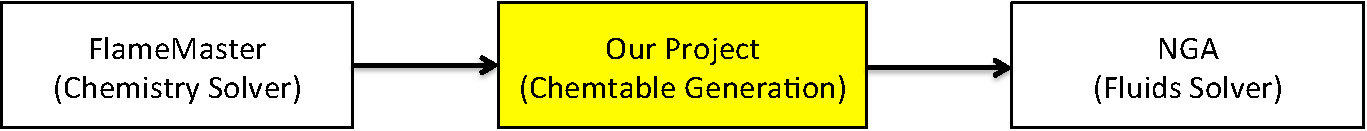
\includegraphics[width=\textwidth]{scope}
\caption{\label{fig:overview} Context of project in relation to existing research codes.}
\end{figure}

Our project uses outputs from an existing research code called
FlameMaster to facilitate and automate the selection of progress
variables. Our project also processes output data from FlameMaster to
create a chemtable through sorting based on the selected progress
variable, convoluting, and interpolating. A variety of interpolation
schemes, integration methods, and PDFs are incorporated into the code
to ensure that it is easily adaptable. The automated selection of
progress variable has not been implemented in any existing
code. Furthermore, although there does exist code to create chemtables
after the progress variable has been defined, it lacks generality and
must be rewritten or substantially modified when requirements for the
chemtable change. A modular program for this task developed with a
well-defined interfaces will significantly improve the generality and
usability of the chemtable code.

\section{Design Process}
The design process for this project began with identifying
deficiencies in existing combustion research codes used by the
Computation Reacting Turbulent Flow Laboratory (CTRFL). We identified
several routines that could be made modular: sorting, integrating,
interpolating, and PDFs. Next, we outlined the overall process of our
software by drawing flowcharts (Fig.~\ref{fig:flow1} and
~\ref{fig:flow2}). This also helped structure our interfaces, as the
flowcharts helped us identify inputs and outputs of the various
routines. During the process of determining the steps of our program,
we deliberated “make versus buy” decisions. After identifying which
routines could take advantage of polymorphism, we examined the
strengths of programming languages covered during lectures and decided
that C++ was best for data processing and computation-heavy functions
that may be parallelized. Python is selected to be the data messenger
between C++ functions, since it can interface with C++ and allows
plots of results to be generated quickly. Before writing any code, we
determined how information needed to flow between each routine, and
designed concrete interfaces for our code. Only a few minor changes
were required to the interfaces as the program developed.

Increasing the amount of functionality by intermediate milestones has
presented us the opportunity to receive feedback from the class and
improve future iterations of our program as well as ensure our project
can achieve its core goals. Specifics on the tools used during the
design process (such as for testing and profiling) are provided in the
“Architecture” section.

\subsection{Make vs. Buy}
Many routines used exist in external libraries (e.g. interpolators,
integrators, PDFs). The decision to write original codes versus use
libraries was determined by the simplicity of routine, our interfaces,
and the expected performance time.

For simple integrators and interpolators, original codes were
written. Some of the more complicated routines (e.g. quadrature
integration or Hermite interpolation) use orthogonal polynomials that
are far more challenging to write and test, so the external library
AlgLib was used.

Interfaces posed a slight problem for the PDFs. In our design review,
it was suggested that we use external libraries to calculate values
for the Beta PDF. This could have worked if we calculated PDF values
on the fly during convolution. Instead, our approach required knowing
full distributions over a range of statistics. It was far easier to
calculate numerous PDF values at once and store them in a matrix.

Lastly, original routines had negligible influence on the total
runtime (see Profiling). In terms of runtime, there is little benefit
to using better-optimized, professionally-written code.
 
\section{Architecture}
Our project consists of two related parts: determining the best
progress variable (Fig.~\ref{fig:flow1}) and generating the chemtables
(Fig.~\ref{fig:flow2}). Our program is based in C++. SWIG is used to
interface the C++ functions with Python. Python 2.7 will be used. The
following tools are used during software development:

\begin{itemize}
\item Tests are implemented using Python Unittest as functionality is
  added throughout the development process.
\item Documentation of the program is performed using Doxygen.
\item Git is used for version control.
\item Valgrind is used for memory leak checks.
\item cProfile is utilized for profiling.
\end{itemize}

\begin{figure} [h]
\centering
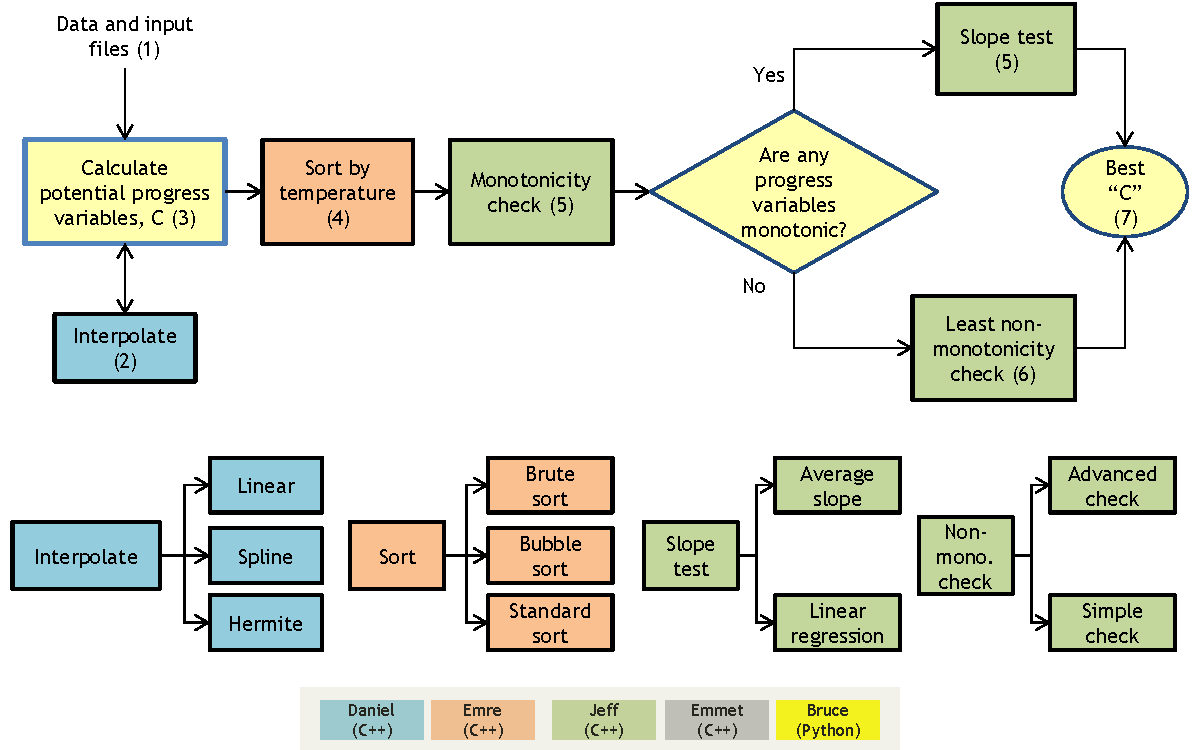
\includegraphics[width=\textwidth]{diagram_1_shortened_v4}
\caption{\label{fig:flow1} Flowchart for progress variable selection. Yellow boxes indicate tasks that will be accomplished in Python and while all other blocks indicate tasks that will be accomplished with C++ functions.}
\end{figure}

\begin{figure} [h]
\centering
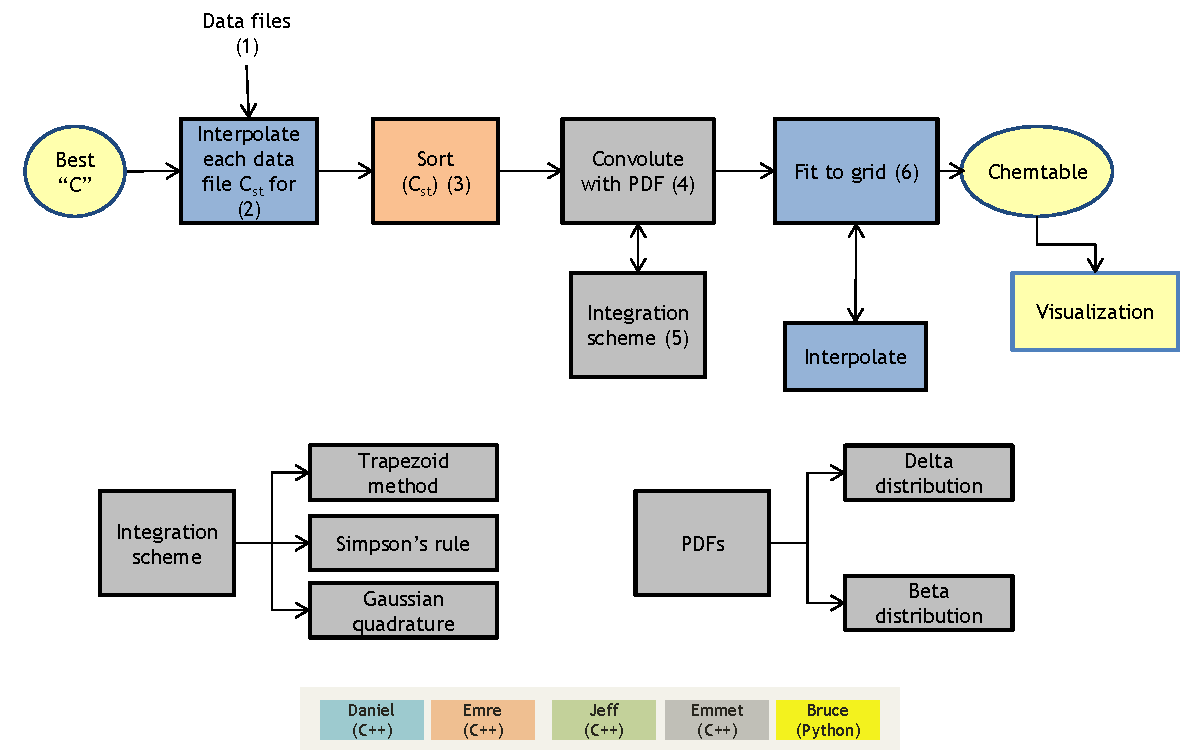
\includegraphics[width=\textwidth]{diagram_2_shortened_v4}
\caption{\label{fig:flow2} Flowchart for generating the chemtables, using the progress variable  determined by the first section of code. All functions for this section of the program will be written in C++ and called from a Python program that provides the user interface.}
\end{figure}

\subsection{Progress Variable, $C$}
As shown in Fig.~\ref{fig:flow1}, inputs to the progress variable
section of our program include a text input file containing the user’s
selection of options to be used during run time and many combustion
data files containing thermochemical state information. The final
output in Fig.~\ref{fig:flow1} is the best progress variable, which is
passed to the table generation section of our program in
Fig.~\ref{fig:flow2}. Detailed descriptions of the processes in
Fig.~\ref{fig:flow1} are below.

\begin{enumerate} 
\item Input files contain a user-specified stoichiometric mixture
  fraction value, a user-specified list of species mass fractions, and
  a set of full thermochemical states represented as columns of
  temperature, species mass fraction, and chemical source terms in
  mixture fraction space. All combinations of mass fractions in the
  user-specified list are candidates for the progress variable.
\item Python code exports two rows from each thermochemical state to
  be interpolated at the stoichiometric mixture fraction.
\item Python code calculates all progress variable candidates at these
  interpolated values.
\item C++ code sorts all progress variables by the stoichiometric
  temperature through various sort functions, generating arrays of
  temperature and all progress variables. These arrays are the only
  data used for the rest of this section.
\item All progress variables are tested for monotonicity with
  temperature in C++ code.
\item Monotonic progress variables will be ranked by various tests,
  \textit{e.g.} an average slope test.
\item If no monotonic progress variables exist, the variables will be
  tested to pick the one that is least non-monotonic, \textit{e.g.}
  monotonic over the greatest range.
\item The best progress variable will be sent to the table generation
  section.
\end{enumerate}

\subsection{Table Generation}
The table generation portion of our project is shown in
Fig.~\ref{fig:flow2}.  Inputs include the best progress variable from
the previous section, thermochemical states (data files), a grid input
file, and a text input file containing the user’s selection of options
to be used during run time (same text input file from
Fig.~\ref{fig:flow1}).  The final output of this part of the code is a
chemtable, which can be fed into another program for further
processing.  Detailed descriptions of the processes in
Fig.~\ref{fig:flow2} are below.


\begin{enumerate}
\item The input data files are the same inputs used for the progress
  variable selection. The best progress variable, as determined by the
  processes depicted in Fig.~\ref{fig:flow1}, is also an input.
\item Progress variable is calculated for each data file and
  interpolated to find the value at the stoichiometric mixture
  fraction $C_{st}$. Various interpolation schemes are used in the
  required sections of the program. User selection of the
  interpolation methods for each process is determined from the text
  input file which contains the chosen scheme.
\item The data files are sorted by the stoichiometric progress
  variable, again using inheritance and polymorphism for the sorting
  functions. The algorithm used is read from the text input file.
\item Numerical integration schemes are used in the convolution step.
  Like interpolation and sorting, these numerical integration schemes
  exploit inheritance and polymorphism. Again, the numerical
  integration scheme is determined by the user in the text input file.
\item The progress variable is convoluted with PDFs. The user
  specifies which PDF to use for convolution.  The implementation is
  polymorphic and the PDF to be used is specified in the text input
  file.  The output is an array of values to be passed to the next
  process.
\item These values are interpolated onto a table (grid) that is
  specified by the grid input file.  This is the chemtable that is the
  final output of our program.
\end{enumerate}

\subsection{Implemented Routines}
Several of the steps in both section of the program are conducive to
polymorphism - for example, specific styles of interpolation are
employed as classes which inherit from an abstract interpolation
class. Multiple integration methods, sorting schemes, and probability
density functions are implemented in a similar manner. The polymorphic
classes that we use in our code in different sections are listed here.

\subsubsection{Sort}
\begin{itemize}
\item “Brute” sort 
\item Bubble sort
\item C++ Standard Library
\end{itemize}

\subsubsection{Integration}
\begin{itemize}
\item Trapezoidal method
\item Simpson’s rule
\item Gauss-Legendre quadrature
\end{itemize}

\subsubsection{Interpolation}
\begin{itemize}
\item Linear
\item Cubic spline
\item Hermite Interpolation
\end{itemize}

\subsubsection{Probability Density Function}
\begin{itemize}
\item Delta function
\item Beta distribution
\end{itemize}


\subsection{External Functions}

We have used the following outside functions and packages to
facilitate the development of our software:
\begin{itemize} 
\item C++ Standard Library
\item Numpy - matrix and vector calculations in Python
\item Matplotlib - contour plots of chemtable results
\item SWIG - interface between Python and C++
\item Numpy.i - SWIG typemapping
\item FlameMaster (existing research software) - our code will not
  interact with FlameMaster, but the data files (*.kg) generated by
  FlameMaster will serve as inputs to our code
\end{itemize}

\subsection{Utilization of SWIG: Python - C++ Interface}
C++ is interfaced with Python using SWIG. SWIG is the interface
compiler that connects C - C++ functions with scripting languages like
Python, Perl or Ruby. We have implemented the wrapper for our separate
routines as depicted in Fig.  \ref{fig:swig}. This figure represents
the python wrapping of the integrator module as an
example. Compilation with SWIG generates *\_wrap.cxx, *.py and *.so
files. Generated shared objects can be imported by a Python script and
the routines written in C++ can be called from the Python file.

\begin{figure} [h]
\centering
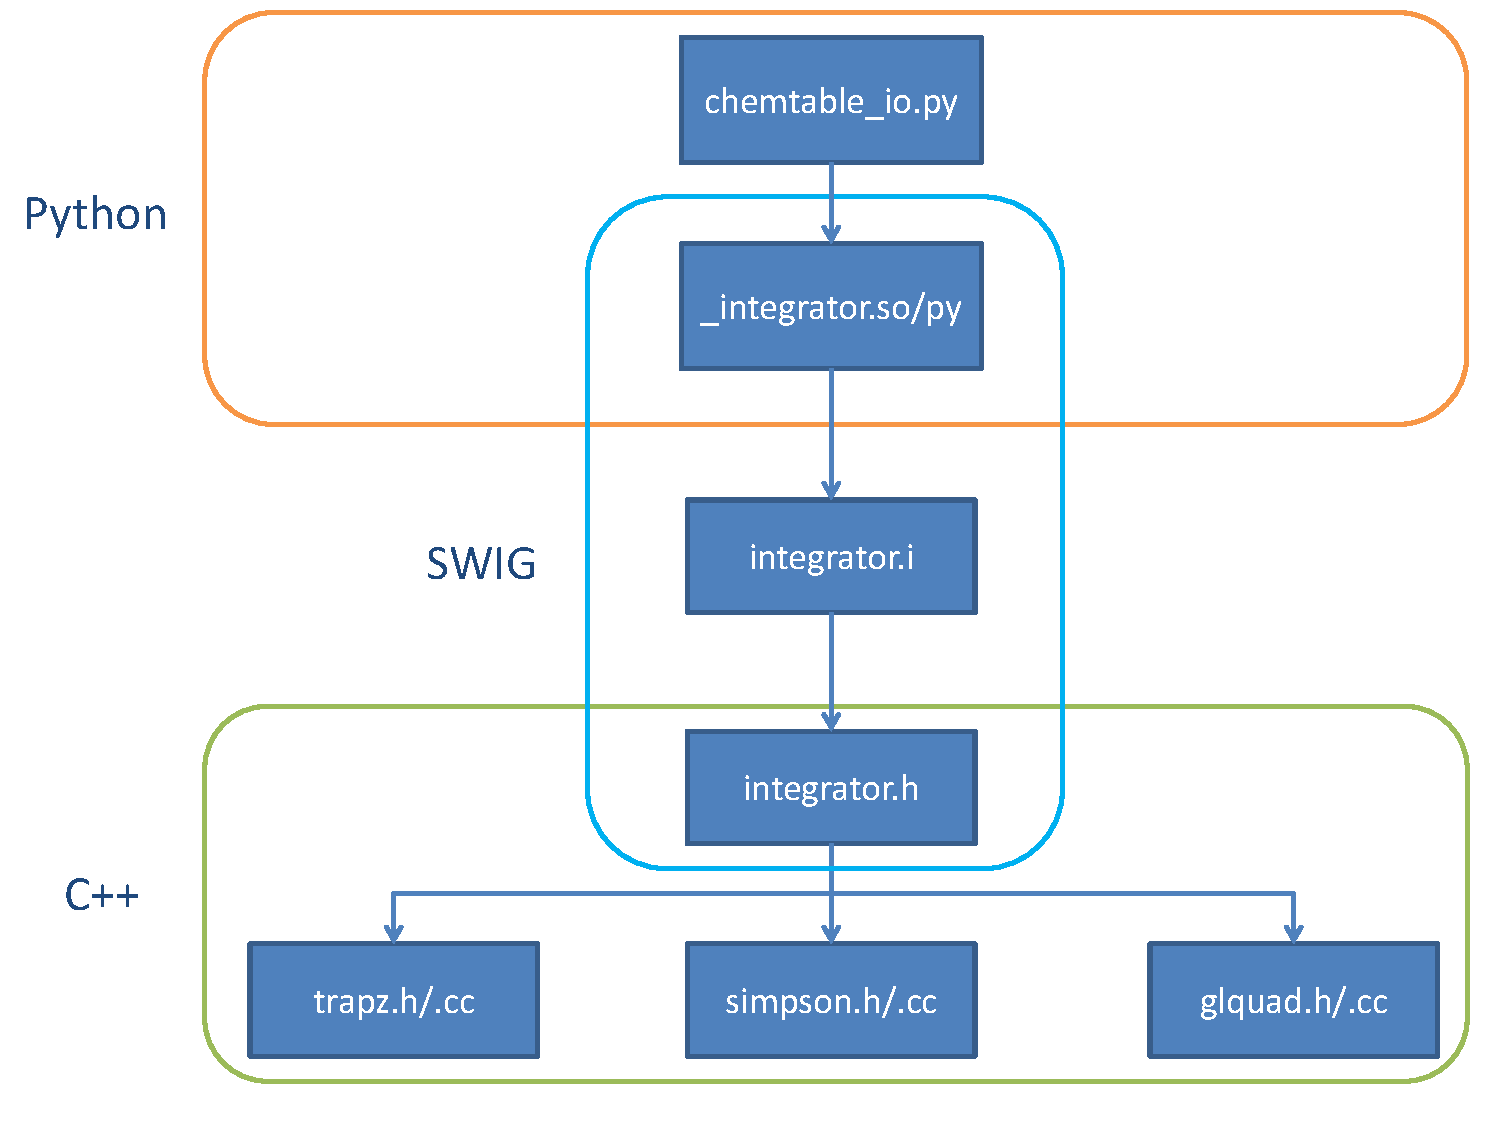
\includegraphics[width=0.7\textwidth]{python_swig_c++}
\caption{\label{fig:swig} Role of SWIG in interface between Python and C++ as shown through the integrator example.}
\end{figure}


\section{Versions}

\subsection{Prototype - 12/5/2014}
This version included at least one derived class from each step working separately. C++ code was compiled separately and no Makefiles were submitted. A primitive demo of reading flamelet files, creating candidate progress variables, and plotting was also included.
%\begin{itemize}
%\item Interface between functions (All)
%\item Interpolation routines (Daniel)
%\item Sorting algorithms (Emre, Jeffry)
%\item Monotonicity check and maximum slope tests (Bruce, Jeffry)
%\item Integration schemes (Emmet, Daniel)
%\item Probability density functions (Emmet)
%\item I/O text processing (Emre, Bruce)
%\end{itemize}
\\
\subsection{Alpha version - 12/12/2014}
This version included C++ code for at least one derived class per
abstract class. SWIG was used to create one module per derived
class. SWIG typecasting was done using standard vectors. All code was
compiled using separate Makefiles for each derived class, each called
by a single executable bash script. Python code interacts with a text
input file, calls each module accordingly and prints out tabulated
data in the terminal.
%\begin{itemize}
%\item Preliminary Python wrapper will be implemented using SWIG and will allow for some %user interaction. (Emre, Emmet) 
%\item One routine from each step (1 interpolator, 1 sorting algorithm, the basic monotonicity %check, maximum slope check, 1 integration scheme along with 1 PDF) will be implemented %in C++. (All)
%\item The link between the progress variable selection and chemtable generation sections %will be implemented with Python. (Daniel, Jeffry)
%\item Fully-functional program that works on well-behaved data sets. (All)
%\item Basic plotting capability will be incorporated for visualization of the preliminary results.  %(Bruce)
%\end{itemize}

\subsection{Beta version - 01/15/2015}
All derived classes were written. SWIG now generates one module per
abstract class. Python code interacts with a text input file, uses
full data sets, calls each module accordingly, prints out tabulated
data in a text file, and generates contour plots of the tabulated
data. All C++ and Python code were tested using Python UnitTest. All
files are organized in separate directories containing source code,
objects, modules, test functions, data, and output. All code is now
compiled from a single Makefile. Parallelization using OpenMP was
implemented reduce runtimes of FitToGrid.
%\begin{itemize}
%\item Fully-operational Python wrapper allows for autonomous and
%  interactive use.
%\item Based on the interface we will already have built for the alpha
%  function, we will implement alternative functions for
%  interpolation, least non-monotonicity checking, integration, PDFs,
%  and sorting.
%\item Fully-functional program that works on real FlameMaster output
%  data.
%\item Interactive and advanced plotting capabilities will be
%  incorporated for visualization.
%\item Error-checking functionality.
%\item Speed of key functions will be optimized.
%\end{itemize}

%For the beta version each team member will extend their own sections
% from the prototype %and alpha version.

\section{Division of Work and Git Repository Log}
Figures~\ref{fig:flow1} and~\ref{fig:flow2} show C++/Python codes were
divided among the group. Each team member was responsible for testing
his own code. There were several other tasks done by all team members:
\begin{itemize}
\item Swig interface files (*.i)
\item Test functions
\item Alpha version Makefiles
\item Design Document/Reports/Presentations
\end{itemize}
SWIG interface files were particularly hard to write, especially for
our implementation (for abstract classes rather than derived
classes). As our project critically depended on making this work, all
team members spent large amounts of time learning SWIG for the Alpha
version. Specifically, Daniel made a breakthrough by implementing
numpy.i for type-recasting. This first appears in only lininterp.i in
the Alpha version, and was adopted for all SWIG interface files for
the Beta version. Emmet made a breakthrough in generating modules for
abstract classes, rather than generating modules for derived
classes. Again, this format was adapted by all for the Beta version.

Other tasks were assigned to individual team members:
\begin{itemize}
\item DOxygen documentation: Emre
\item Beta version Makefiles: Emmet
\item Beta version README: Bruce
\end{itemize}

There are discrepancies between team members in the Git repository
commit log. We attribute this to various styles of using Git. Bruce
and Emmet frequently committed minor changes to the repository, while
Daniel committed code larger sections of code more infrequently.

\section{Results}

The chemtable generation program has been successfully applied to two
data sets: a complete set of FlameMaster outputs for combustion of
C2H4, and a truncated subset of this data chosen to be a
“well-behaved” test case. These datasets were chosen to be
representative of real data that would be analyzed to make a chemtable
in turbulent combustion research. The input files used to run these
example cases are shown in Appendix A. Additionally, the outputs
printed by the program to the terminal when running these cases are
shown in Appendix B. Note that a warning is printed that the input
“plot all progress variables:” has not been specified and the default
value, “yes”, is being used.

Figure \ref{fig:xa_xb} shows the results of the progress variable
selection portion of the program, using the simplified and full data
sets, respectively. The species examined for inclusion in the progress
variable are H2O, H2, CO2, and OH. For the truncated data case, almost
all candidate progress variables increase monotonically with
temperature, and the program selects the candidate with the maximum
slope (Y-H2O + Y-H2 + Y-CO2 + Y-OH). The program prints out this
progress variable and lists separately all other monotonically
increasing progress variables. For the complex case, all progress
variables are non-monotonic, and the program correctly identifies the
non-monotonic progress variable which is non-monotonic over the
smallest range (Y-H2O + Y-H2 + Y-CO2). In fact, the non-monotonic
region is small enough to be indistinguishable in
Fig. \ref{fig:xa_xb}(b). Still, the program prints out a warning that
no completely monotonically increasing progress variable was found.

\begin{figure} [h]
\centering
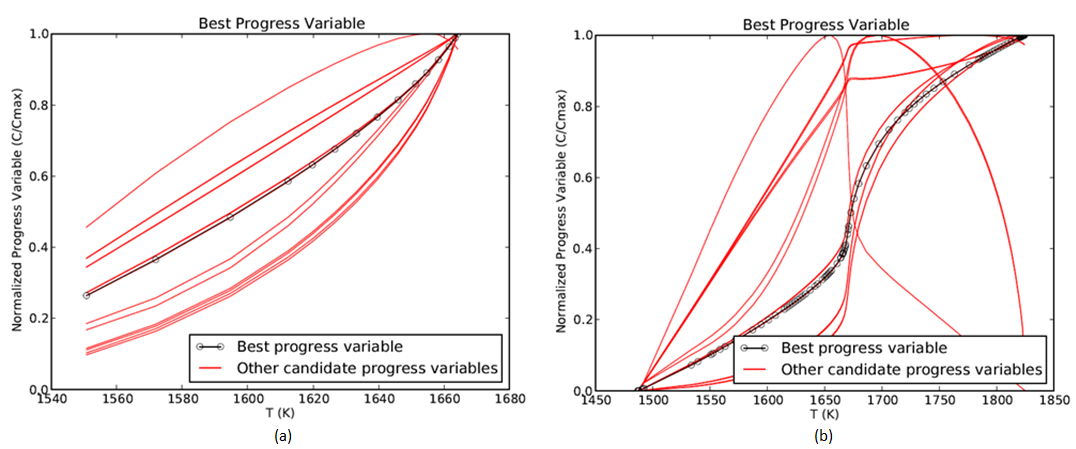
\includegraphics[width=\textwidth]{xa_xb.PNG}
\caption{\label{fig:xa_xb} Plots of the selected progress variable and
  other candidate progress variables as a function of temperature for
  the (a) truncated and (b) full data sets.  }
\end{figure}

Figure \ref{fig:ya_yb} shows sample contour plots generated from the
truncated and full data. The contour plot generated from the truncated
data matches expectations for how chemical source term should depend
on these variables for canonical combustion systems (Knudsen E, Pitsch
H. Combust Flame 156 (2009) 678–696). The contour plot for the full
data set is qualitatively similar, but has artifacts near where there
are large gradients in chemical source term. These artifacts are a
result of the slight non-monotonicity in the chosen progress variable
and are unavoidable. Overall, these plots show that the chemtable
generation program performs as expected and the data it produces is
reliable.

\begin{figure} [h]
\centering
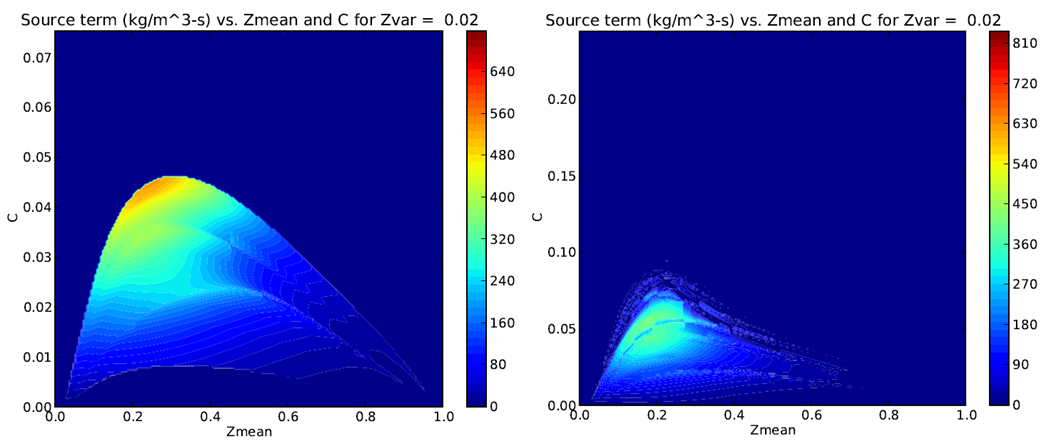
\includegraphics[width=\textwidth]{ya_yb.PNG}
\caption{\label{fig:ya_yb} Contour plots of chemical source term as a
  function of progress variable (C) and mixture fraction (Zmean) at
  Zvar = 0.02 for the (a) truncated and (b) full data sets.}
\end{figure}

\subsection{Profiling}
Profiling our code was done using cProfile. For all cases, we used
reasonable numbers of flamelets (data files inputs) as well a grid
sizes.

Our results point to FitToGrid as the bottleneck in our code. Results
from tests with 201 grid points for Zmean and Cgrid, and 26 grid
points for Zvar took FitToGrid 126 s to run and the entire program 142
s. FitToGrid performs two tasks, namely interpolation and
extrapolation. We attribute the long runtimes to the extrapolation
part of this function, which contains 5 nested for loops. These for
loops are necessary to search through a 3-dimensional matrix, and then
for each point, to search through the same matrix again for the
point’s nearest neighbor. Our only choice to speed up this part of the
code was through parallelizing these loops. We chose to parallelize
using OpenMP for its simplicity. Furthermore, even after all future
work is implemented (see future work section), our expected runtime
should not exceed several hours. This runtime is negligible compared
to any LES that will use these chemtables, so parallelizing with MPI
to use >16 nodes was deemed unnecessary.

Fig. \ref{fig:fittogrid} shows runtimes using 1, 2, 4, and 8
threads. Again, grid sizes were taken to be 201 points for Zmean and
Cgrid, and 26 points for Zvar. For all cases, the total runtime is
about 16 s longer than the FitToGrid times. For 1, 2, and 4 threads
used, FitToGrid times roughly decrease by half as the number of
threads doubles, indicating an $\mathcal{O}(n^{-1})$ dependence on
thread number, as expected. The times for 8 threads deviates from this
trends simply because the cost of parallelizing to 8 threads becomes
comparable to the speedup.

\begin{figure} [h]
\centering
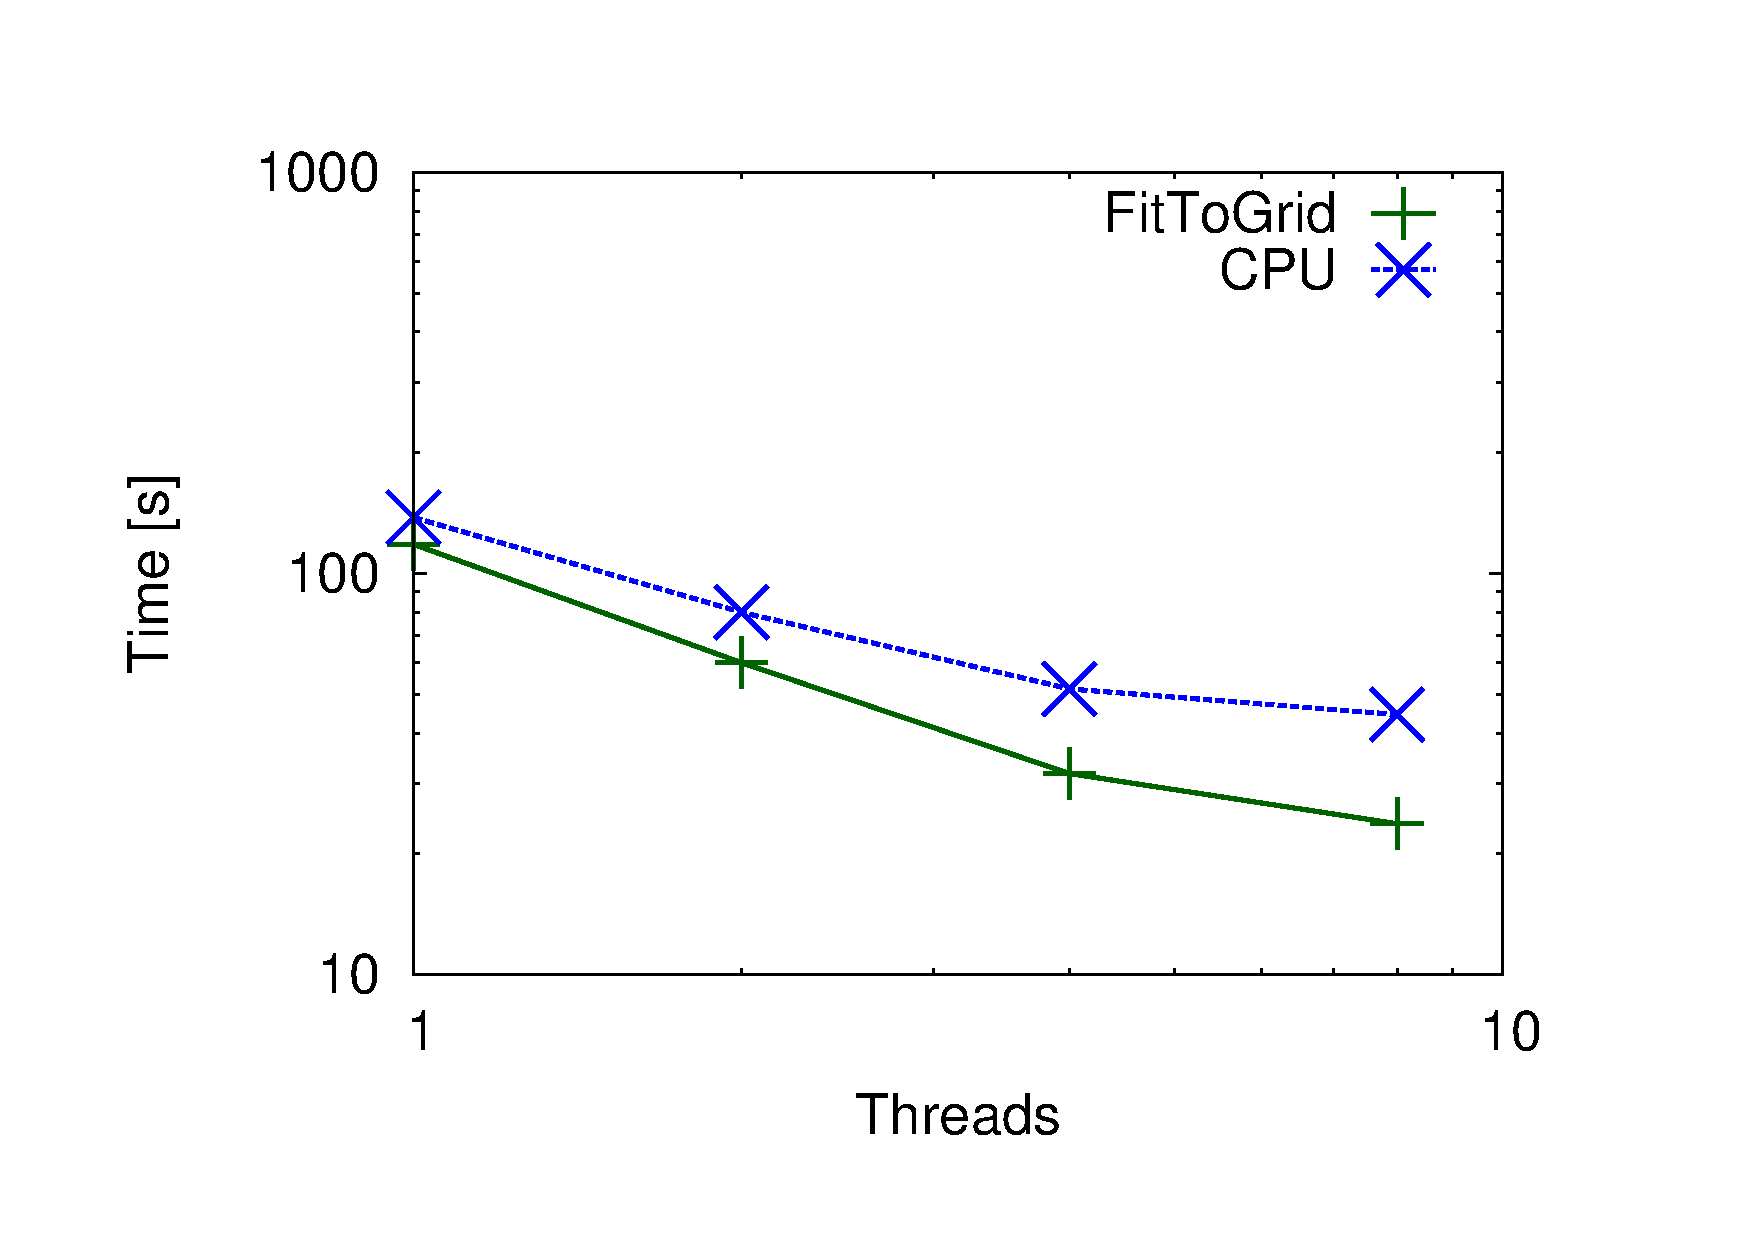
\includegraphics[width=0.6\textwidth]{plot_threads}
\caption{\label{fig:fittogrid} Comparison of runtimes for FitToGrid
  and total runtime (CPU).}
\end{figure}

\begin{figure} [h]
\centering
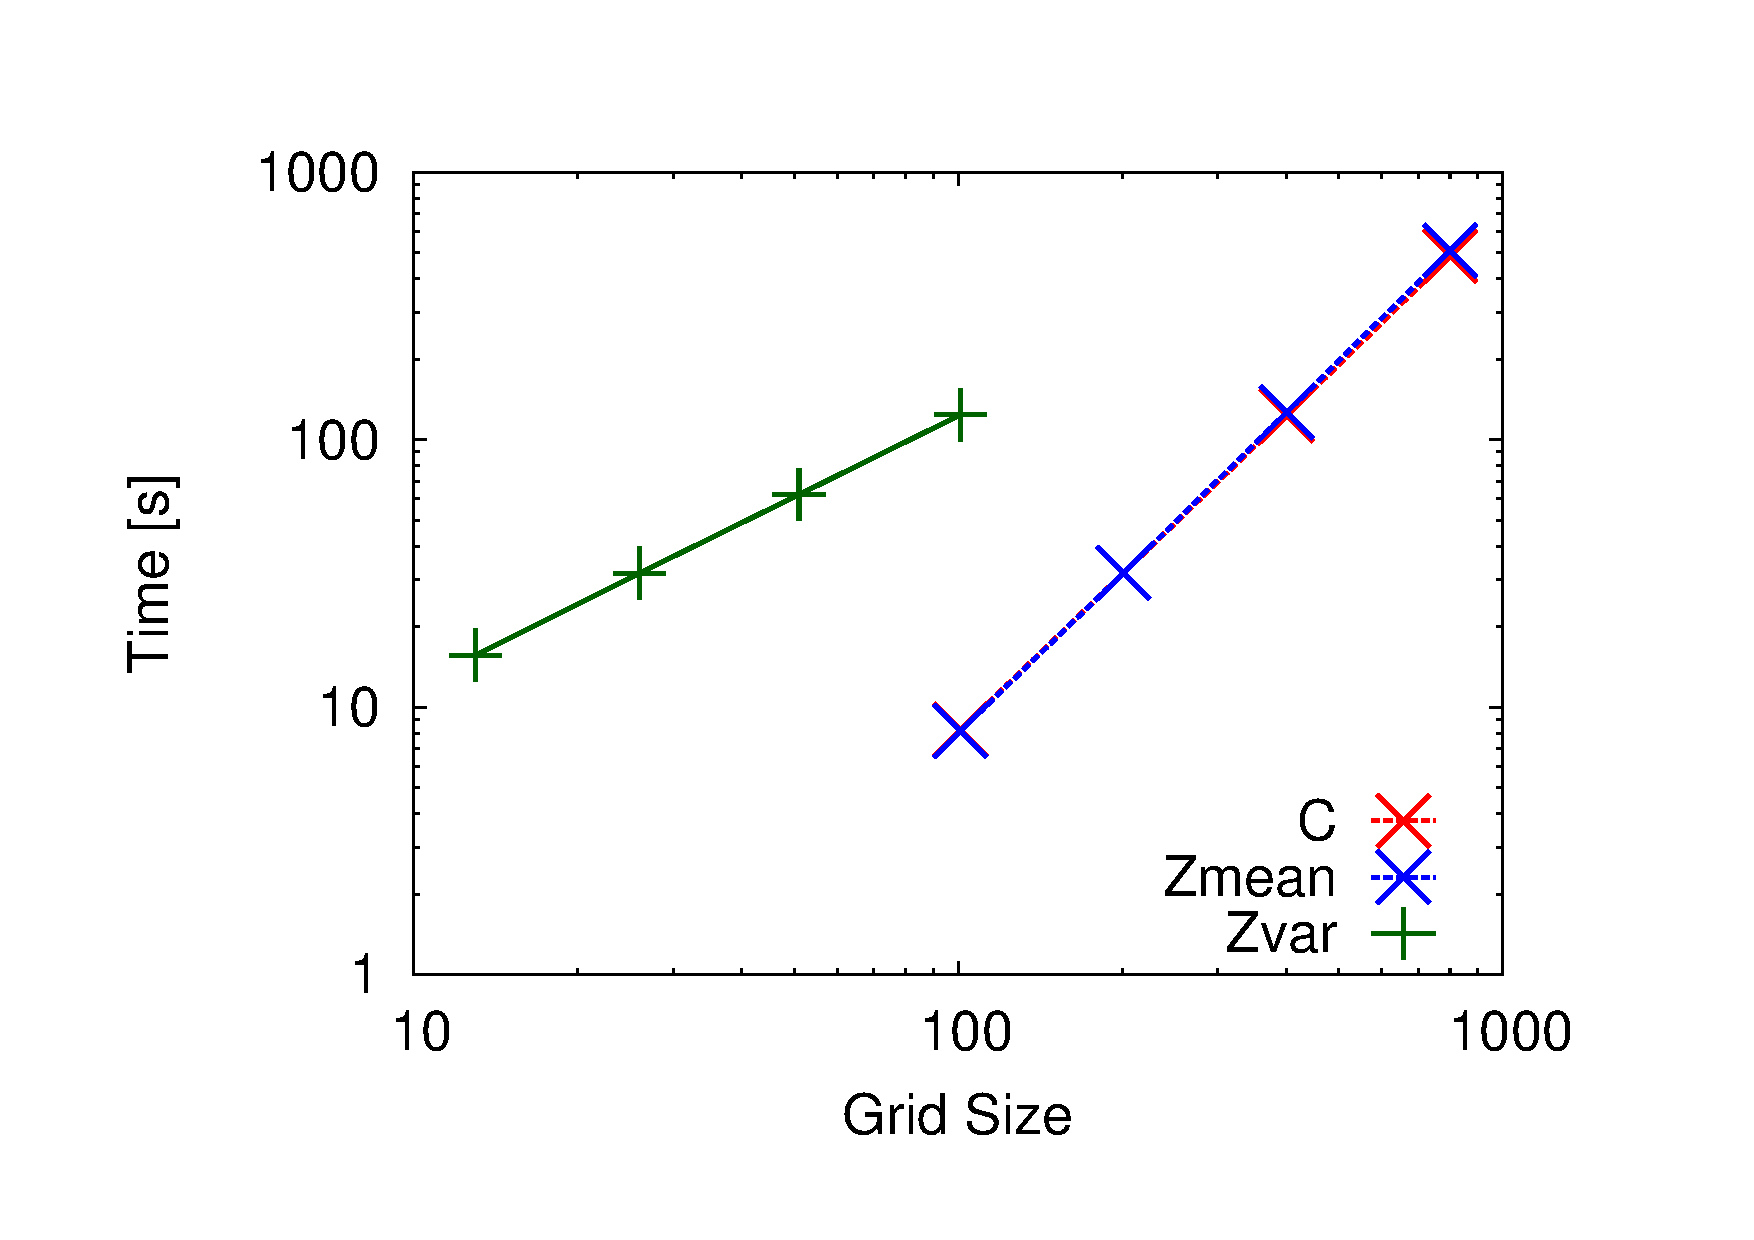
\includegraphics[width=0.6\textwidth]{plot_gridsizes}
\caption{\label{fig:gridsensitivity} Sensitivity of parallelized code
  to grid size.}
\end{figure}

\subsection{Performance of Interpolators}
Using linear interpolation gave results which made sense, but Hermite
and cubic interpolation gave nonsensical results in some cases. An
illustrative example is shown in figure~\ref{fig:interpolator}. Steep
gradients in the data cause the interpolating polynomials to have
steep gradients as well, leading to the nonsensical results
observed. Linear interpolation is, of course, insensitive to such
effects. This leads us to question the appropriateness of
interpolation schemes which are susceptible to such effects.

\begin{figure} [h]
\centering
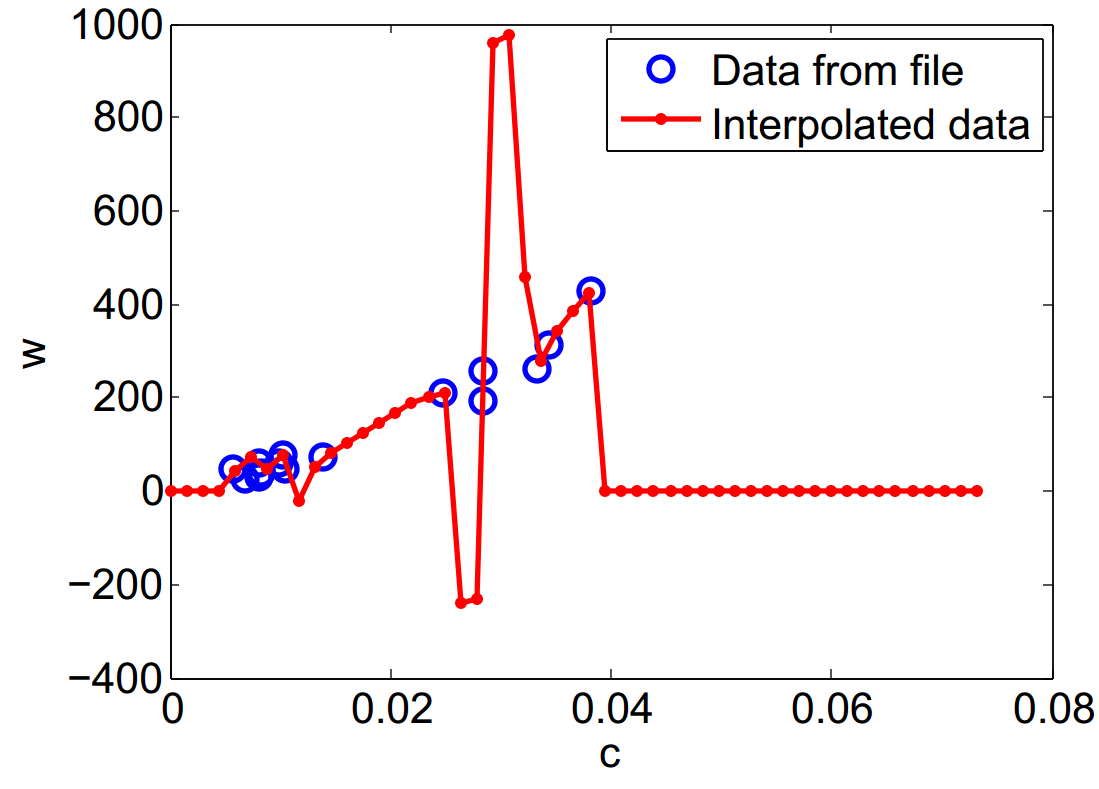
\includegraphics[width=0.6\textwidth]{interpolator.PNG}
\caption{\label{fig:interpolator} Interpolating along a grid using
  cubic Hermite interpolation.}
\end{figure}

%\section{Future Work}
%Identifying a truly bijective mapping between progress variable and
% thermochemical state is among the most challenging and arbitrary
% parts of turbulent combustion simulations using flamelet
% models. This software greatly facilitates the progress variable
% selection process and will likely be used by researchers in the
% Computational Turbulent Reacting Flow Laboratory (CTRFL). While this
% software does meet all of our project objectives, there is future
% work to be done.

%\begin{itemize}
%\item Software should be extended to filter all chemical species
%  individually in addition to filtering chemical source terms as it
%  already does. Only filtered chemical source terms are needed to run
%  LES, but filtered species mass fractions and temperature are needed
%  for visualization of LES results.
%\item Mathematically rigorous algorithms for finding the least
%  non-monotonic progress variable can be incorporated based on current
%  mathematics research. For example, an index of
%  non-decreasingness\footnote{Qoyyimi \textit{et al.}, SSRN. (2014),
%    pp. 1-23.} can be implemented. Their applicability to progress
%  variable selection is, to date, unknown, but would be an interesting
%  topic of research.
%\item Manual selection of the best progress variable from a plot
%  generated at the end of the section shown in
%  Fig.~\ref{fig:flow1}. Currently, our program allows manual selection
%  of the best progress variable at the very beginning, where the user
%  is unable to view all the possible options.
%\end{itemize}

% We also think that the runtime of our code may be an issue for large
% data sets and for the cases which require large number progress
% variable candidates. Also for our research purposes, the data sets
% that our program will deal with are considerably large. If time
% turns out to be a bigger issue, we may consider implementing
% multi-threading parallelization using OpenMP.

% Identifying a truly bijective mapping between progress variable and
% thermochemical state is among the most challenging and arbitrary
% parts of turbulent combustion simulations using flamelet
% models. Furthermore, even perfectly monotonic progress variables may
% have wildly varying slopes over temperature, so the highest average
% slope may not necessarily give the best progress variable. In fact,
% one may not even exist. For our project to be incorporated into real
% research codes it must still be able to deal with these challenging
% situations. In the worst cases, this can only be dealt with through
% plotting numerous graphs and requiring the user to visually
% determine the best progress variable. Regardless, our code will
% still greatly facilitate this process.

% Both sections of our project are independently useful. Even if one
% is not successful, our project will still provide a useful tool for
% turbulent combustion simulations. And due to the modular structure
% of our project, even if one component cannot be completed, the
% remaining portions will not be affected by this
% problem. Furthermore, the modular structure of our project allows us
% to develop the various components in parallel and iterate rapidly
% through versions of our code.

\section{What We Learned}
For most team members, this project was their first experience coding
collaboratively. This was no easy feat: version control and interface
design are particularly challenging in collaborative projects. We
benefitted greatly from designing our interfaces early in the design
process and sticking to them, and using a Git Repository greatly
facilitated sharing and debugging code.

This was also our first experience working on a project with so many
files. This was incredibly hard and confusing to maintain for the
Alpha version, and would have been even worse for the Beta version had
we not sorted our source code, modules, test, etc. into different
directories. Thus, we also learned the value of maintaining a clean
and organized working directory.

None of our team members had ever interfaced languages. This part of
the project was probably the most troublesome to get working. SWIG was
difficult to learn, but was incredibly useful. By interfacing C++ with
python, we were able to handle IO text processing in python, as well
as test our C++ code using python UnitTest.

\section{Conclusion/Future Work}
Identifying a truly bijective mapping between progress variable and
thermochemical state is among the most challenging and arbitrary parts
of turbulent combustion simulations using flamelet models. This
software greatly facilitates the progress variable selection process
and will likely be used by researchers in the Computational Turbulent
Reacting Flow Laboratory (CTRFL). While this software does meet all of
our project objectives, there remains future work that could further
enhance the functionality and usability of this code:

\begin{itemize}
\item Software should be extended to filter all chemical species
  individually in addition to filtering chemical source terms as it
  already does. Only filtered chemical source terms are needed to run
  LES, but filtered species mass fractions and temperature are needed
  for visualization of LES results.
\item Mathematically rigorous algorithms for finding the least
  non-monotonic progress variable can be incorporated based on current
  mathematics research. For example, an index of
  non-decreasingness\footnote{Qoyyimi \textit{et al.}, SSRN. (2014),
    pp. 1-23.} can be implemented. Their applicability to progress
  variable selection is, to date, unknown, but would be an interesting
  topic of research.
\item Manual selection of the best progress variable from a plot
  generated at the end of the section shown in
  Fig.~\ref{fig:flow1}. Currently, our program allows manual selection
  of the best progress variable at the very beginning, where the user
  is unable to view all the possible options.
\end{itemize}


\clearpage
\section*{Appendix A: Input File}

The input file used to run the sample cases described in the Results
section is shown below. This input file is for the full case, but the
input file for the truncated case is identical except that “data/C2H4”
is replaced by “data/C2H4truncated”.

\vspace{12pt}


\hfill\begin{minipage}{\dimexpr\textwidth-3cm}
data file directory:	data/C2H4 \\
test species:	Y-H2O	Y-H2	Y-CO2	Y-OH \\
output file name:	data\_out \\
plot all progress variables:	\\
skip progress variable optimization:	no \\
extrapolate in fittogrid:	no \\
\\
number of threads:	4 \\
\\
Zmean\_grid:	201 \\
Zvar\_max:	0.25 \\ 
Zvar\_grid:	26 \\
\\
Zpdf:	beta \\
sort method:	standard \\
StoichMassFrac:	0.05 \\ 
interp method:	linear \\ 
max slope test:	linear regression \\
integrator:	trapezoid \\
least nonmonotonic check:	simple \\

glq Number of Nodes:	10 \\
length Cgrid:	201 \\

\xdef\tpd{\the\prevdepth}
\end{minipage}


\clearpage
\section*{Appendix B: Output}

Output for the full data case:
\vspace{12pt}


\hfill\begin{minipage}{\dimexpr\textwidth-3cm}

using default input for plot all progress variables:
['yes'] \\
Sorting PROGVARS by temperature using standard sort \\
Sorting FILESMATRIX by temperature \\
Testing monotonicity  \\
\\
Finding least non-monotonic progress variable using simple nonmono check \\
WARNING: no monotonic progress variables found, but proceeding with best alternative. \\
\\
The least non-monotonic progress variable is C = Y-H2O + Y-H2 + Y-CO2 \\ 
The column numbers of these species are [8, 7, 9] , respectively. \\
\\
\\
Sorting filesmatrix by C using standard sort\\
Generating PDF matrix with beta PDF\\
PDF calculated\\
Convoluting using trapezoid integration\\
Convolution completed\\
Maximum value of progress variable is: 0.162988071\\
Fitting final data to grid using linear interpolation\\
No extrapolation used to fit to grid\\
\\
Final data written to file: output/data\_out \\
10 contour plots created in output directory \\

\xdef\tpd{\the\prevdepth}
\end{minipage}

\vspace{12pt}


\newpage
Output for the truncated data case:
\vspace{12pt}

\hfill\begin{minipage}{\dimexpr\textwidth-3cm}


using default input for plot all progress variables:
['yes'] \\
Sorting PROGVARS by temperature using standard sort\\
Sorting FILESMATRIX by temperature\\
Testing monotonicity \\
\\
Testing max slope using linear regression\\
The chosen progress variable is C = Y-H2O + Y-H2 + Y-CO2 + Y-OH \\
The column numbers of these species are  [8, 7, 9, 6] , respectively.\\
\\
Other candidate monotonic progress variables are:\\
C = Y-H2O \\
C = Y-CO2 \\
C = Y-OH \\
C = Y-H2O + Y-H2 \\ 
C = Y-H2O + Y-CO2 \\
C = Y-H2O + Y-OH \\
C = Y-H2 + Y-CO2 \\
C = Y-H2 + Y-OH \\
C = Y-CO2 + Y-OH \\
C = Y-H2O + Y-H2 + Y-CO2 \\ 
C = Y-H2O + Y-H2 + Y-OH \\
C = Y-H2O + Y-CO2 + Y-OH \\
C = Y-H2 + Y-CO2 + Y-OH \\
\\
Sorting filesmatrix by C using standard sort\\
Generating PDF matrix with beta PDF\\
PDF calculated\\
Convoluting using trapezoid integration\\
Convolution completed\\
Maximum value of progress variable is: 0.050205925\\
Fitting final data to grid using linear interpolation\\
No extrapolation used to fit to grid\\
\\
Final data written to file: output/data\_out\\
10 contour plots created in output directory 

\xdef\tpd{\the\prevdepth}
\end{minipage}



\end{document}


 
